% Search for all the places that say "PUT SOMETHING HERE".

\documentclass[11pt]{article}
\usepackage{amsmath,textcomp,amssymb,geometry,graphicx,enumerate}

\usepackage [english]{babel}
\usepackage [autostyle, english = american]{csquotes}
\def\Name{Quoc Thai Nguyen Truong}  % Your name
\def\SID{24547327}  % Your student ID number
\def\Login{cs161-di} % Your login (your class account, cs170-xy)
\def\Homework{2}%Number of Homework
\def\Session{Spring 2015}


\title{CS161--Spring 2015 --- Solutions to Homework \Homework}
\author{\Name, SID \SID, \texttt{\Login}}
\markboth{CS161--\Session\  Homework \Homework\ \Name}{CS161--\Session\ Homework \Homework\ \Name, \texttt{\Login}}
\pagestyle{myheadings}

\newenvironment{qparts}{\begin{enumerate}[{(}a{)}]}{\end{enumerate}}
\def\endproofmark{$\Box$}
\newenvironment{proof}{\par{\bf Proof}:}{\endproofmark\smallskip}

\textheight=9in
\textwidth=6.5in
\topmargin=-.75in
\oddsidemargin=0.25in
\evensidemargin=0.25in

\newcommand{\tab}{\hspace*{2em}}


\begin{document}
\maketitle

Collaborators: God

\section*{Problem 1}

\begin{qparts}
\item
$$c'_2 = 0\ \ ,\ \ d'_2 = 0$$
$$c'_{3t} = c_3\ \ ,\ \ d'_{3t} = min(d_3,b_3)$$
$$c'_{3f} = max(a_3 + 1,c_3)\ \ ,\ \  d'_{3f} = d_3$$
$$c'_4 = c_4\ \ ,\ \ d'_4 = d_4$$
$$c'_5 = c_5 + 1\ \ ,\ \ d'_5 = c_5 + 1$$
\\
\item
$$c_3 = min(c'_2,c'_5)\ \ ,\ \ d_3 = max(d'_2,d'_5)$$
$$c_6 = min(c'_{3f},c'_{1f})\ \ ,\ \ d_6 = max(d'_{3f},d'_{1f})$$
\\
\item
The vulnerability of the function is \boxed{Off\ By\ One}
\end{qparts}


\newpage
\section*{Problem 2}
\begin{qparts}
\item
\boxed{Failsafe\ defaults}
\\
The default is not unsafe to give \$300 to customer without checking card is valid or not.
\item
\boxed{complete\ mediation}
\\
It should check for authority in every users/objects before let them access the web.

\item
\boxed{Security\ through\ obscurity}
\\
A system relying on security through obscurity may have theoretical or actual security vulnerabilities. Since the duress code is known through public documentation, the attacker can find and attack.
\item
\boxed{Least\ privilege}
\\
The SuperFlashlight controls and access the information and recourse that are not necessary for legitimate purpose.
\end{qparts}
\newpage
\section*{Problem 3}

\begin{qparts}
\item
\boxed{NO}
\\
Since Bob does not have root access, so he can't execute escalate.c .

\item
\boxed{YES}
\\
Since we know that other users can able to run the file with the privileges of the owner, Bob will able to execute escalate.c .

\item
\boxed{YES}
\\
Once he got the path of the file, he can call new$\_$event on that path so  that it can make a copied of the file and execute escalate.c .

\end{qparts}


\newpage
\section*{Problem 4}

\begin{qparts}
\item
\boxed{False}
\\
It can be very effective but cannot defend against malware unless some of its samples have already been obtained, a proper signatures generated and the antivirus product updated.
Also, this does not really effective against zero-day or next-generation malware.
\item
\boxed{True}
\\
Advertising, by definition, is ceding control of Web content to another party

\item
\boxed{False}
\\
Rootkit is a set of trojan system binaries.It can install hacked binaries for system programs such as netstat, ps, ls, du, login

\item
\boxed{True}


\end{qparts}

\newpage
\section*{Problem 5}

Repeat "http://browsertest.com/?u=" after "/?u="\\
http://browsertest.com/?u= http://browsertest.com/?u= http://browsertest.com/?u= ... \\
\\
If there are n repetitions and n is large, BrowerTest will make $2^n$ HTTP requests. Therefore, this will overload the BrowerTest server.

\newpage
\section*{Problem 6}

\begin{enumerate}

\item
\begin{qparts}
\item
\boxed{Blacklisting}
\\
$+$One Advantage: it is conceptually simple to recognize a few bad things(virus, malware), stop them, and allow everything else.
\\\\
$+$One disadvantage: Very hard to capture the malicious string as we can see in the project, and it's not a good practice if it allows attacker to use an attribute from html form to perform an XSS attack.
\\

\item
\boxed{YES}
\\
Example: If an attacker entering malicoous user-name which contains "scrscriptipt....", the library will remove substring "script". Therefore it becomes "script..." . 
\end{qparts}

\item
\begin{qparts}
\item
This is Cross Site Request Forgery (CSRF) vulnerability, or one-click attack. Eva stole one dollar from me by let me click on the tinyrul and the Tinyrul redirect to:\\
http://www.cashbo.com/payment?amount=1$\&$recipient=Eve\\
Now, I lost 1 dollar.\\
\item
For every transaction, we should ask the user to re-enter their username and password to make sure that he/she is authorized current user.
\end{qparts}

\end{enumerate} 

\newpage
\section*{Problem 7}


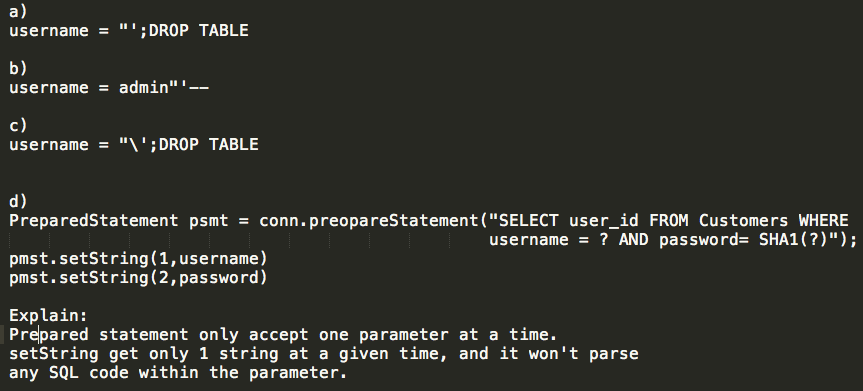
\includegraphics[scale=0.5]{7abcd.png}


e)
\newpage
\section*{Problem 8}
Great!!!

\end{document}
